\documentclass[12pt]{extarticle}
\usepackage[margin=30pt]{geometry}
\usepackage{amsmath}
\usepackage[slovak]{babel}
\usepackage[T1]{fontenc}
\usepackage{multicol}
\usepackage{graphicx}
\graphicspath{ {../assets/} }
\usepackage{tikz}
\usepackage{pgfplots}
\pgfplotsset{
	table/search path={../assets/},
}

\title{%
Laboratórna práca č.1\\
Izotermický dej
}
\author{}
\date{}

\begin{document}
\begin{titlepage}
	\maketitle
	\thispagestyle{empty}
	\vfill
	\large
	\begin{tabular}{ll}
		Dátum merania: 21.12.2023 \hfill &Meno: Adam Labuš \\
		Spolupracovníci: Pavol Medveczký, Martin Németh &Trieda: Sexta B \\
	\end{tabular}
	\vspace{100pt}
\end{titlepage}

\def\present#1#2{%
	\begin{samepage}
	{\large #1}\\
	\begin{center}
		#2\\[1em]
	\end{center}
	\end{samepage}
}

\def\graf#1#2{
	\present{#1}{
		\begin{tikzpicture}
			#2
		\end{tikzpicture}
	}
}

\section{Postup}
\begin{enumerate}
\item Coach panel zapojíme do počítača.
\item Do Coachu zapojíme tlakový senzor.
\item Do tlakového senzoru zapojíme hadičku a na jej druhý koniec zapojíme striekačku s objemom 20ml.
\item Na počítači si zvolíme aký sme použili senzor a nakalibrujeme ho na aktuálny atmosferický tlak 1009,5hPa.
.
\item Postupne stláčame striekačku, zapisujeme jej objem a hodnotu zo senzora. Spolu sme urobili 14 meraní.
\item Prvý graf, ktorý urobíme je tlak v závislosti od objemu.
\item Na druhý graf potrebujem najprv pridať do tabuľky nový stĺpec, ktorého hodnoty budú podľa vzorca $p * V$. Graf nastavíme tak aby x-ová os bola číslo merania a y-ová os bola z nášho novo vytvoreného stĺpca. Hodnota konštanty v Boyleovom-Mariottovom zákone je na grafe vidieť na y-ovej osi.
\item Na tretí graf znovu vytvoríme nový stĺpec v tabuľke, tentokrát podľa vzorca $1/V$. Nastavíme x-ovú os grafu na $p$, y-ová os na $1/V$.
\item Posledný graf ofitujeme lineárnou funkciou.
\end{enumerate}

\section{Namerané a vypočítané hodnoty}
\present{Screenshot po meraní}{
	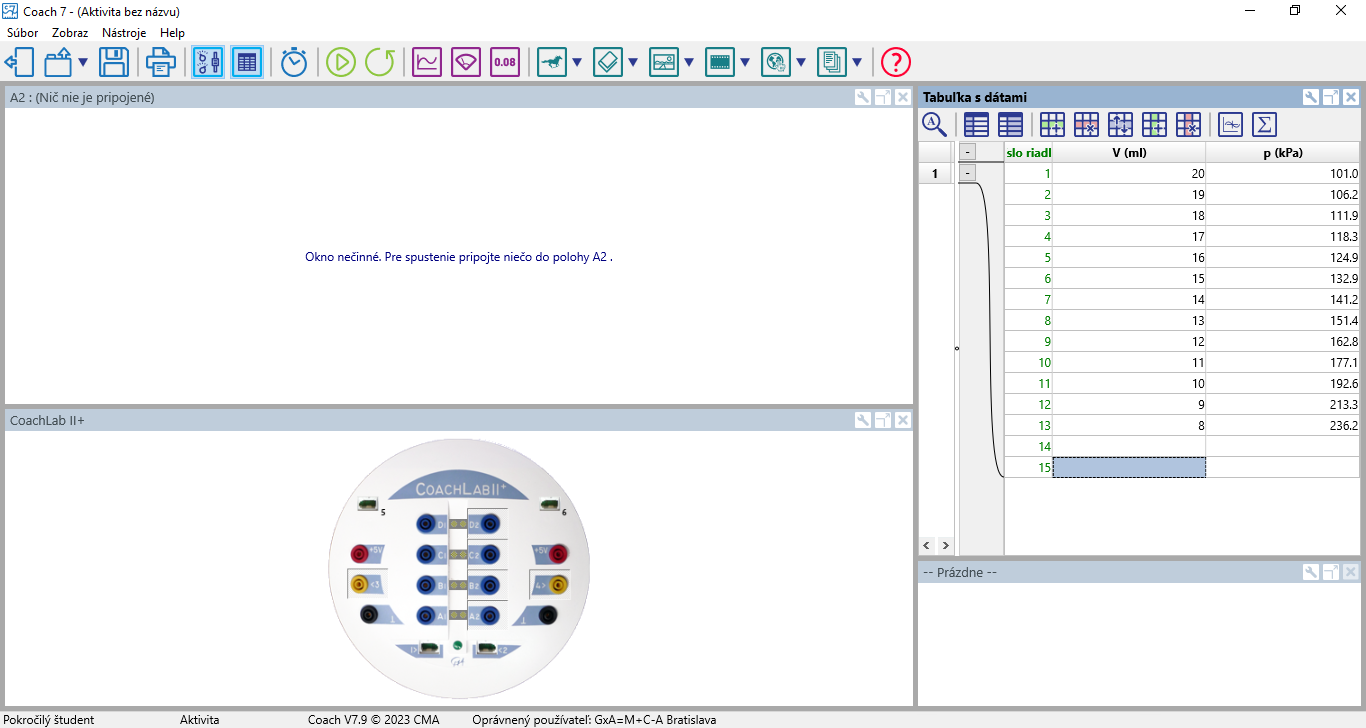
\includegraphics[width=0.8\textwidth]{fullscreen}
}
\graf{Graf I., tlak v závislosti od objemu}{%
	\begin{axis}[y label style={rotate=270}, xlabel={V[ml]}, ylabel={p[kPa]}, ymin=0]
		\addplot table [x=x, y=y, col sep=comma] {p_od_V.csv};
	\end{axis}
}

\graf{Graf II., tlak krát objem v závislosti od čísla merania}{%
	\begin{axis}[y label style={rotate=270}, xlabel={Číslo merania}, ylabel={(pV)[kPa * ml]}, ymin=0]
		\addplot table [x=x, y=y, col sep=comma] {pV_od_cisla_merania.csv};
	\end{axis}
}

\graf{Graf III., tlak v závislosti od recipročnej hodnoty objemu}{
	\begin{axis}[y label style={rotate=270}, xlabel={(1/V)[1/ml]}, ylabel={p[kPa]}, ymin=0]
		\addplot table [x=x, y=y, col sep=comma] {p_od_1_deleno_V.csv};
	\end{axis}
}

\graf{Graf IV., tlak v závislosti od recipročnej hodnoty objemu s ofitovanou funkciou }{
	\begin{axis}[y label style={rotate=270}, xlabel={(1/V)[1/ml]}, ylabel={p[kPa]}, ymin=0]
		\addplot table [x=x, y=y, col sep=comma] {p_od_1_deleno_V.csv};
		\addplot[color=red, thick][domain=0.02:0.14]{1808.91 * x + 11.69};
	\end{axis}
}
{\begin{center} \large $a = 1808.91$ \end{center}}

\section{Záver}
\begin{enumerate}
\item Pozorovali sme izotermický dej lebo: \\[1em]
$\frac{p * V}{T}$ = konštanta\\[1em]
Z nášho pozorvania vieme, že $p * V$ je tiež konštantná hodnota. Znamená, že platí: \\[1em]
$\frac{konštanta}{T}$ = konštanta\\
$T =$ konštanta\\[1em]
To, že tlak krát objem je konštanta ($p* V =$ konštanta) sa nazyvá Boylov-Mariottov zákon. Jeho celé slovné znenie je: \textit{Pri izotermickom deji s ideálnym plynom so stálou hmotnosťou je súčin tlaku a objemu plynu stály.} \cite{zakon}
\item
V grafe I je vidieť nepriama úmernosť medzi tlakom voči objemu, lebo graf klesá a je zakrivený v strede tak ako to vidíme v lomenej funkcií.
\item Na grafe II je skoro vodorovná čiara, teda konštantná funkcia.
Je to lebo platí Boyleov-Marriotov zákon. Hovorím "skoro vodorovná čiara", lebo ako už bolo spomenuté Boyleov-Marriotov zákon platí pre \textbf{ideálny plyn}, vzduch ním nie je.
Tým, že sčítame všetky hodnoty v tomto grafe a vydelíme ho počtom meraní, zistíme, že hodnota našej konštanty je približne $1.831[kPa * l]$.
\end{enumerate}

\begin{thebibliography}{3}
	\bibitem{zakon}
	https://sk.wikipedia.org/wiki/Boylov-Mariottov\_z\%C3\%A1kon
\end{thebibliography}

\end{document}
